% A path gamma from gamma(0) to gamma(1) inside a space X (blob), with an
% arrow indicating direction of travel.
% Source: book/tex/topology/top-more.tex (§ Path-connectedness).
\documentclass[border=2mm]{standalone}
\usepackage{tikz}
\usetikzlibrary{arrows.meta}
\begin{document}
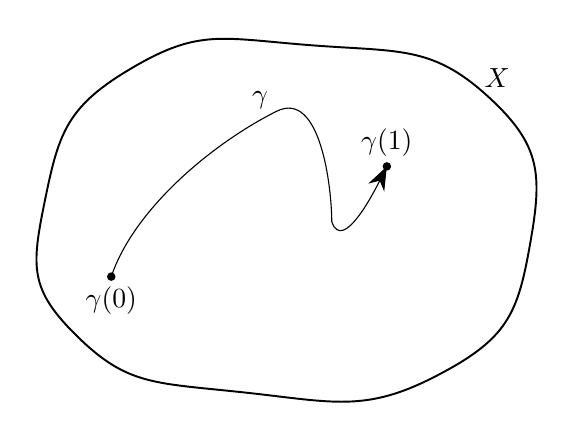
\begin{tikzpicture}[scale=0.7]
  \draw[black, line width=0.7pt]
    plot[smooth cycle, tension=0.9]
    coordinates {(-4.2,0.4) (-2.6,2.8) (0.6,3.2) (3.8,2.3) (4.6,-0.4)
                 (2.9,-2.8) (-0.6,-3.1) (-3.6,-2.1)};
  \node at (4.0,2.6) {$X$};
  \fill (-3,-1) circle (2.2pt) node[below] {$\gamma(0)$};
  \fill (2,1) circle (2.2pt) node[above] {$\gamma(1)$};
  \draw[-{Stealth[length=3mm]}]
    (-3,-1) .. controls (-2.6,0.2) and (-1.2,1.4) .. (0,2)
            .. controls (0.8,2.4) and (1.0,0.6) .. (1,0)
            .. controls (1.2,-0.6) and (1.8,0.6) .. (2,1);
  \node at (-0.3,2.2) {$\gamma$};
\end{tikzpicture}
\end{document}
